%%%%%%%%%%%%%%%%%%%%% chapter04.tex %%%%%%%%%%%%%%%%%%%%%%%%%%%%%%%%%
%
% Chapter 4: Model Formats and Quantization
%
%%%%%%%%%%%%%%%%%%%%%%%% Springer-Verlag %%%%%%%%%%%%%%%%%%%%%%%%%%

\chapter{Model Formats and Quantization}
\label{ch:models}

\abstract*{The choice of model format and quantization level directly impacts performance, quality, and resource requirements. This chapter explains the major model formats (SafeTensors, GGUF, ONNX), demystifies quantization techniques (GPTQ, AWQ, GGML/GGUF), provides guidance on choosing models for different use cases, and introduces the concept of a model registry for your control plane. We focus on the practical knowledge needed to make informed model selection decisions.}

\abstract{The choice of model format and quantization level directly impacts performance, quality, and resource requirements. This chapter explains the major model formats (SafeTensors, GGUF, ONNX), demystifies quantization techniques (GPTQ, AWQ, GGML/GGUF), provides guidance on choosing models for different use cases, and introduces the concept of a model registry for your control plane. We focus on the practical knowledge needed to make informed model selection decisions.}

% =============================================================================
\section{Understanding Model Formats}
\label{sec:model-formats}
% =============================================================================

Chapter~\ref{ch:hardware-fundamentals} showed us how to calculate VRAM requirements: a 7B model at FP16 needs 14 GB, but quantized to INT4 needs only 3.5 GB. But where do these quantized models come from? How do you choose between the dozens of variants on Hugging Face? This chapter answers these questions.

The path from a trained model to inference involves several decisions: which format to use (SafeTensors, GGUF, ONNX), which quantization method (GPTQ, AWQ, GGUF's built-in quantization), and which specific quantization level (Q4, Q5, Q8). Each choice affects memory usage, inference speed, and output quality. By the end of this chapter, you'll know how to navigate these options and select the right model for your hardware and use case.

Before examining specific formats, we need to understand what a model file must contain and the principles that guide format design. Whether you're loading models, building inference engines, or even designing a new format, these fundamentals apply.

\subsection{What a Model File Contains}
\label{subsec:model-contents}

A neural network model file must store everything needed to reconstruct the model's computation graph and execute inference. At minimum, this includes:

\begin{description}
\item[Weight Tensors] The learned parameters---billions of floating-point numbers organized into matrices. A 7B model contains approximately 7 billion of these values across hundreds of individual tensors (one per layer component: attention projections, feed-forward layers, embeddings, etc.).

\item[Tensor Metadata] The shape, data type, and name of each tensor. Without knowing that \texttt{layers.0.attention.wq} is a $[4096 \times 4096]$ matrix of FP16 values, the raw bytes are meaningless.

\item[Model Architecture] How tensors connect: number of layers, attention heads, hidden dimensions, vocabulary size. Some formats embed this; others rely on external configuration files.

\item[Tokenizer] (Optional) The vocabulary and encoding rules that convert text to token IDs. Often stored separately but sometimes bundled.
\end{description}

% Diagram: Inference Engine Pipeline
% Shows the flow from request to response through engine components

\begin{figure}[htbp]
\centering
\begin{tikzpicture}[
    node distance=1.2cm and 1.5cm,
    box/.style={rectangle, draw, rounded corners, minimum width=2.2cm, minimum height=1cm, align=center, font=\small},
    arrow/.style={->, thick, >=stealth},
    label/.style={font=\footnotesize\itshape, text=gray}
]

% Top row: Input processing
\node[box, fill=blue!10] (request) {Request\\Handler};
\node[box, fill=green!10, right=of request] (tokenizer) {Tokenizer};
\node[box, fill=orange!10, right=of tokenizer] (forward) {Forward\\Pass};

% Bottom row: Output generation
\node[box, fill=purple!10, below=of forward] (kvcache) {KV Cache\\Manager};
\node[box, fill=red!10, below=of tokenizer] (sampler) {Sampler};
\node[box, fill=blue!10, below=of request] (response) {Response\\Streamer};

% Top row arrows
\draw[arrow] (request) -- (tokenizer);
\draw[arrow] (tokenizer) -- (forward);

% Down and across
\draw[arrow] (forward) -- (kvcache);
\draw[arrow] (kvcache) -- (sampler);
\draw[arrow] (sampler) -- (response);

% Loop back for autoregressive generation (curved path on the right side)
\draw[arrow, dashed, rounded corners=8pt]
    (kvcache.east) -- ++(0.8,0) -- ++(0,1.2) -- ++(-0.8,0) -- (forward.east);
\node[label, anchor=west] at ($(kvcache.east) + (0.9, 0.6)$) {next token};

% Input/Output labels
\node[left=0.5cm of request, font=\small] (input) {``Hello''};
\node[left=0.5cm of response, font=\small] (output) {``Hi!''};
\draw[arrow] (input) -- (request);
\draw[arrow] (response) -- (output);

% Component labels
\node[above=0.15cm of request, label] {API/Queue};
\node[above=0.15cm of tokenizer, label] {Text $\rightarrow$ IDs};
\node[above=0.15cm of forward, label] {GPU Compute};
\node[below=0.15cm of kvcache, label] {Memory Mgmt};
\node[below=0.15cm of sampler, label] {Token Select};
\node[below=0.15cm of response, label] {SSE Stream};

\end{tikzpicture}
\caption{Inference engine pipeline. Requests flow through tokenization and the forward pass (top row), then through KV cache management and sampling (bottom row). The dashed arrow shows the autoregressive loop---each generated token feeds back through the forward pass until generation completes.}
\label{fig:inference-pipeline}
\end{figure}


\subsection{How Architecture Connects to Weights}
\label{subsec:architecture-weights}

A critical distinction exists between \emph{weights-only} formats (SafeTensors, GGUF) and \emph{graph-embedded} formats (ONNX). Understanding this clarifies how inference actually works.

\paragraph{Weights-Only Formats: Code Defines the Graph}

SafeTensors and GGUF store tensors with names like \texttt{model.layers.0.self\_attn.q\_proj.weight}. These names follow conventions, but the file contains no instructions for how to use them. The computation graph---what operations to perform and in what order---lives in code.

When you load a Llama model:
\begin{enumerate}
\item The inference engine reads architecture metadata (number of layers, head count, dimensions)
\item It constructs the computation graph in code: ``for each layer, apply attention, then FFN, then residual''
\item It loads weight tensors by name and binds them to the corresponding graph nodes
\item The code defines the forward pass; the weights are just parameters
\end{enumerate}

This is why llama.cpp, vLLM, and Hugging Face Transformers each implement their own model architectures. They all load the same weights, but each has code that knows ``Llama uses RoPE embeddings, GQA attention, and SwiGLU activation.''

For concrete examples, see llama.cpp's Llama implementation\footnote{\url{https://github.com/ggerganov/llama.cpp/blob/master/src/llama.cpp}} or Hugging Face's LlamaModel class\footnote{\url{https://github.com/huggingface/transformers/blob/main/src/transformers/models/llama/modeling_llama.py}}. Both load identical weights but implement the forward pass differently.

\paragraph{Graph-Embedded Formats: Self-Describing Models}

ONNX takes the opposite approach: the file contains both weights \emph{and} a directed acyclic graph (DAG) of operations. Each node specifies an operation (MatMul, Softmax, Add) and references input/output tensors by name.

\begin{svgraybox}
\textbf{Trade-off: Flexibility vs. Portability}

\begin{description}
\item[Weights-only (SafeTensors, GGUF)] Smaller files. Requires engine to implement architecture. Enables engine-specific optimizations (fused kernels, custom attention).

\item[Graph-embedded (ONNX)] Larger files. Any ONNX runtime can execute without architecture knowledge. Limited to operations the runtime supports.
\end{description}

For LLMs, weights-only formats dominate because engines like vLLM implement heavily optimized, architecture-specific kernels that outperform generic graph execution.
\end{svgraybox}

\paragraph{Concrete Example: Llama 3.2 7B Architecture}

Let's trace how weights map to computation for a real model. Llama 3.2 7B has:
\begin{itemize}
\item \textbf{32 transformer layers}, each containing attention and feed-forward blocks
\item \textbf{4096 hidden dimension} (the size of vectors flowing through the model)
\item \textbf{32 attention heads} with \textbf{8 KV heads} (Grouped Query Attention)
\item \textbf{14336 intermediate dimension} for the feed-forward network
\item \textbf{128k vocabulary} for the embedding and output layers
\end{itemize}

Each layer contains these weight tensors:

\begin{table}[htbp]
\centering
\caption{Weight tensors in one Llama 3.2 7B transformer layer.}
\label{tab:layer-weights}
\begin{tabular}{llrr}
\toprule
\textbf{Component} & \textbf{Tensor} & \textbf{Shape} & \textbf{Size (FP16)} \\
\midrule
Attention & \texttt{q\_proj} & $[4096, 4096]$ & 32 MB \\
          & \texttt{k\_proj} & $[4096, 1024]$ & 8 MB \\
          & \texttt{v\_proj} & $[4096, 1024]$ & 8 MB \\
          & \texttt{o\_proj} & $[4096, 4096]$ & 32 MB \\
\midrule
FFN       & \texttt{gate\_proj} & $[4096, 14336]$ & 112 MB \\
          & \texttt{up\_proj} & $[4096, 14336]$ & 112 MB \\
          & \texttt{down\_proj} & $[14336, 4096]$ & 112 MB \\
\midrule
Norms     & \texttt{input\_layernorm} & $[4096]$ & 8 KB \\
          & \texttt{post\_attention\_layernorm} & $[4096]$ & 8 KB \\
\midrule
\multicolumn{2}{l}{\textbf{Total per layer}} & & \textbf{$\sim$416 MB} \\
\bottomrule
\end{tabular}
\end{table}

Multiply by 32 layers: $\sim$13.3 GB. Add embeddings ($\sim$1 GB) and the output head ($\sim$1 GB): approximately 14 GB for the full model at FP16.

\paragraph{GPU Memory During Inference}

When running inference, GPU memory holds more than just weights:

% Diagram: Traditional vs Paged KV Cache Memory
% Shows memory fragmentation problem and how PagedAttention solves it

\begin{figure}[htbp]
\centering
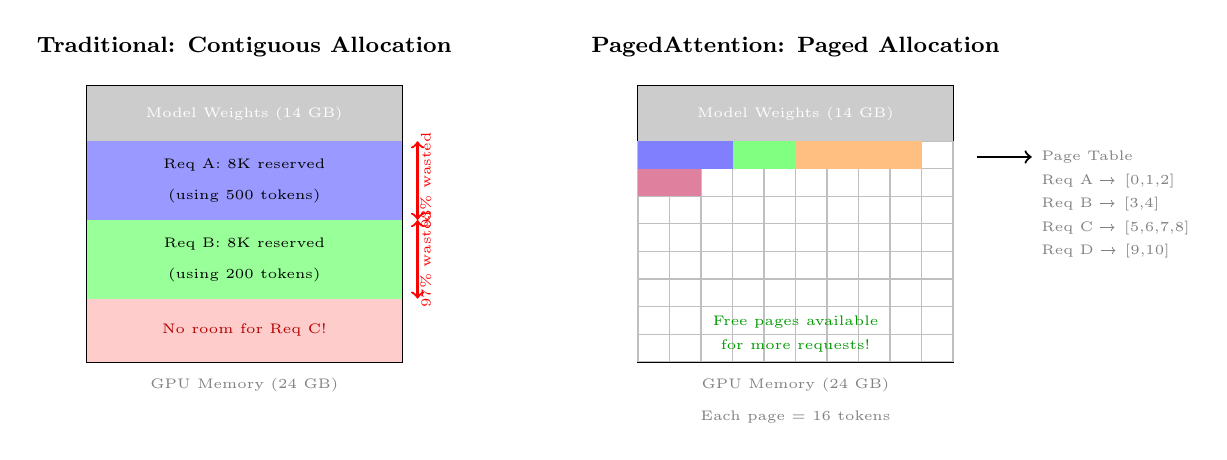
\begin{tikzpicture}[
    node distance=0.2cm,
    memblock/.style={rectangle, draw, minimum height=0.5cm, font=\tiny},
    label/.style={font=\footnotesize},
    timelabel/.style={font=\tiny, text=gray}
]

% === TRADITIONAL ALLOCATION (left) ===
\node[label] at (2, 4) {\textbf{Traditional: Contiguous Allocation}};

% GPU Memory block
\draw[thick] (0, 0) rectangle (4, 3.5);
\node[timelabel] at (2, -0.3) {GPU Memory (24 GB)};

% Model weights (fixed)
\fill[gray!40] (0, 2.8) rectangle (4, 3.5);
\node[font=\tiny, white] at (2, 3.15) {Model Weights (14 GB)};

% KV Cache allocations (pre-allocated for max length)
\fill[blue!40] (0, 1.8) rectangle (4, 2.8);
\node[font=\tiny] at (2, 2.5) {Req A: 8K reserved};
\node[font=\tiny] at (2, 2.1) {(using 500 tokens)};

\fill[green!40] (0, 0.8) rectangle (4, 1.8);
\node[font=\tiny] at (2, 1.5) {Req B: 8K reserved};
\node[font=\tiny] at (2, 1.1) {(using 200 tokens)};

% Wasted space indicator
\fill[red!20] (0, 0) rectangle (4, 0.8);
\node[font=\tiny, red!70!black] at (2, 0.4) {No room for Req C!};

% Fragmentation arrows
\draw[<->, red, thick] (4.2, 1.8) -- (4.2, 2.8);
\node[timelabel, red, rotate=90, anchor=south] at (4.5, 2.3) {93\% wasted};

\draw[<->, red, thick] (4.2, 0.8) -- (4.2, 1.8);
\node[timelabel, red, rotate=90, anchor=south] at (4.5, 1.3) {97\% wasted};

% === PAGED ATTENTION (right) ===
\node[label] at (9, 4) {\textbf{PagedAttention: Paged Allocation}};

% GPU Memory block
\draw[thick] (7, 0) rectangle (11, 3.5);
\node[timelabel] at (9, -0.3) {GPU Memory (24 GB)};

% Model weights (fixed)
\fill[gray!40] (7, 2.8) rectangle (11, 3.5);
\node[font=\tiny, white] at (9, 3.15) {Model Weights (14 GB)};

% Page pool - small fixed-size blocks
\foreach \i in {0,1,2,3,4,5,6,7} {
    \foreach \j in {0,1,2,3,4,5,6,7,8,9} {
        \pgfmathsetmacro{\x}{7 + \j * 0.4}
        \pgfmathsetmacro{\y}{0 + \i * 0.35}
        \draw[gray!50] (\x, \y) rectangle (\x + 0.4, \y + 0.35);
    }
}

% Color used pages
% Req A pages (blue) - scattered
\fill[blue!50] (7, 2.45) rectangle (7.4, 2.8);
\fill[blue!50] (7.4, 2.45) rectangle (7.8, 2.8);
\fill[blue!50] (7.8, 2.45) rectangle (8.2, 2.8);

% Req B pages (green) - scattered
\fill[green!50] (8.2, 2.45) rectangle (8.6, 2.8);
\fill[green!50] (8.6, 2.45) rectangle (9.0, 2.8);

% Req C pages (orange) - can now fit!
\fill[orange!50] (9.0, 2.45) rectangle (9.4, 2.8);
\fill[orange!50] (9.4, 2.45) rectangle (9.8, 2.8);
\fill[orange!50] (9.8, 2.45) rectangle (10.2, 2.8);
\fill[orange!50] (10.2, 2.45) rectangle (10.6, 2.8);

% Req D pages (purple)
\fill[purple!50] (7, 2.1) rectangle (7.4, 2.45);
\fill[purple!50] (7.4, 2.1) rectangle (7.8, 2.45);

% Free pages indicator
\node[timelabel, green!60!black] at (9, 0.5) {Free pages available};
\node[timelabel, green!60!black] at (9, 0.2) {for more requests!};

% Legend
\node[timelabel] at (9, -0.7) {Each page = 16 tokens};

% Page table concept
\draw[->, thick] (11.3, 2.6) -- (12, 2.6);
\node[timelabel, anchor=west] at (12, 2.6) {Page Table};
\node[timelabel, anchor=west, font=\tiny] at (12, 2.3) {Req A → [0,1,2]};
\node[timelabel, anchor=west, font=\tiny] at (12, 2.0) {Req B → [3,4]};
\node[timelabel, anchor=west, font=\tiny] at (12, 1.7) {Req C → [5,6,7,8]};
\node[timelabel, anchor=west, font=\tiny] at (12, 1.4) {Req D → [9,10]};

\end{tikzpicture}
\caption{Traditional vs PagedAttention memory management. Left: Contiguous allocation reserves maximum possible space per request, causing fragmentation and limiting concurrent requests. Right: PagedAttention allocates small fixed-size pages on demand, eliminating fragmentation and enabling 2-4x more concurrent requests.}
\label{fig:paged-attention}
\end{figure}


The computation flows through layers sequentially. For each token generated:
\begin{enumerate}
\item \textbf{Embedding lookup}: Token ID $\rightarrow$ 4096-dim vector
\item \textbf{Layer 0--31}: Each layer transforms the hidden state
\begin{itemize}
\item Attention: Query from current state, Keys/Values from KV cache
\item KV cache update: Store new K, V for this position
\item FFN: Two matrix multiplications with SwiGLU activation
\item Residual connections after each block
\end{itemize}
\item \textbf{Output projection}: 4096-dim $\rightarrow$ 128k logits $\rightarrow$ next token
\end{enumerate}

The KV cache grows with context length. At 4096 tokens with FP16 precision:
\[
\text{KV Cache} = 2 \times 32 \times 8 \times 128 \times 4096 \times 2 \approx 0.5 \text{ GB}
\]

At 32K context, this becomes $\sim$4 GB---a significant fraction of total memory.

\subsection{Design Principles for Model Formats}
\label{subsec:format-principles}

Model formats make different trade-offs, but well-designed formats share common principles. Understanding these helps you evaluate formats and predict their behavior.

\paragraph{Principle 1: Separate Metadata from Data}

Tensor metadata (names, shapes, types, byte offsets) should be readable without loading tensor data. This enables:
\begin{itemize}
\item \textbf{Validation}: Check if a model fits in memory before attempting to load it
\item \textbf{Selective loading}: Load only needed layers (useful for distributed inference)
\item \textbf{Inspection}: Tools can examine model structure without gigabytes of I/O
\end{itemize}

Good formats place metadata in a header or index section. Poor formats interleave metadata with data, requiring a full file scan.

\paragraph{Principle 2: Enable Memory-Mapped Access}

Modern formats support \emph{memory mapping} (mmap), where the operating system maps file contents directly into virtual memory. Instead of reading data into a buffer, you access file bytes through memory pointers.

\begin{svgraybox}
\textbf{Why Memory Mapping Matters:}

Without mmap: Load 14 GB file $\rightarrow$ allocate 14 GB RAM $\rightarrow$ copy 14 GB $\rightarrow$ peak usage: 28 GB

With mmap: Map file to address space $\rightarrow$ access pages on demand $\rightarrow$ OS manages caching $\rightarrow$ peak usage: $\sim$14 GB

Memory mapping also enables:
\begin{itemize}
\item Lazy loading: Only read pages actually accessed
\item Shared memory: Multiple processes can share the same mapped file
\item Faster startup: No explicit read/copy step
\end{itemize}
\end{svgraybox}

For mmap to work efficiently, tensor data must be stored contiguously with known offsets. Formats that require decompression or transformation during loading cannot be memory-mapped.

\paragraph{Principle 3: Align Data for Hardware Efficiency}

GPUs and CPUs access memory most efficiently when data is aligned to specific boundaries (typically 16, 32, or 64 bytes). Misaligned access can halve memory bandwidth.

Well-designed formats:
\begin{itemize}
\item Pad tensors to alignment boundaries
\item Store tensors in the memory layout expected by compute kernels (row-major vs column-major)
\item Group tensors by access pattern (all attention weights together, etc.)
\end{itemize}

\paragraph{Principle 4: Support Zero-Copy GPU Transfer}

The ideal path from disk to GPU:
\begin{enumerate}
\item File bytes $\rightarrow$ pinned CPU memory (DMA transfer)
\item Pinned memory $\rightarrow$ GPU VRAM (PCIe/NVLink transfer)
\end{enumerate}

Each copy operation takes time. Formats that require transformation (decompression, type conversion, transposition) add CPU work and memory allocation between these steps. Formats that store data in GPU-ready layout enable direct streaming.

\paragraph{Principle 5: Embed Sufficient Metadata for Inference}

A standalone model file should contain enough information to run inference without external files. This includes:
\begin{itemize}
\item Architecture parameters (layers, heads, dimensions)
\item Special token IDs (BOS, EOS, padding)
\item Quantization parameters (scales, zero-points)
\item RoPE configuration (rotary embedding parameters)
\end{itemize}

Formats that externalize this information (separate \texttt{config.json} files) create deployment complexity and version mismatch risks.

\paragraph{Principle 6: Ensure Safety and Integrity}

Model files should not execute code during loading. They should also detect corruption:
\begin{itemize}
\item \textbf{No executable content}: Pure data formats prevent malicious payloads
\item \textbf{Checksums}: Detect transmission errors or tampering
\item \textbf{Version markers}: Identify format version for backward compatibility
\end{itemize}

% Diagram: Request Flow through Control Plane
% Shows the step-by-step processing of a request

\begin{figure}[htbp]
\centering
\begin{tikzpicture}[
    node distance=0.6cm,
    flowstep/.style={rectangle, draw, rounded corners, minimum width=2.8cm, minimum height=0.7cm, align=center, font=\small},
    arrow/.style={->, thick, >=stealth},
    label/.style={font=\footnotesize\itshape, text=gray}
]

% Left column - Request path
\node[flowstep, fill=blue!15] (req) {1. Request\\Arrives};
\node[flowstep, fill=blue!10, below=of req] (log) {2. Logging\\Middleware};
\node[flowstep, fill=blue!10, below=of log] (metrics1) {3. Metrics\\Middleware};
\node[flowstep, fill=green!15, below=of metrics1] (validate) {4. Validate\\Request};
\node[flowstep, fill=orange!15, below=of validate] (backend) {5. Backend\\Call};

% Right column - Response path
\node[flowstep, fill=orange!15, right=3cm of backend] (process) {6. Process\\Response};
\node[flowstep, fill=purple!15, above=of process] (record) {7. Record\\Metrics};
\node[flowstep, fill=blue!15, above=of record] (resp) {8. Send\\Response};

% Arrows - down the left side
\draw[arrow] (req) -- (log);
\draw[arrow] (log) -- (metrics1);
\draw[arrow] (metrics1) -- (validate);
\draw[arrow] (validate) -- (backend);

% Arrow across to right side
\draw[arrow] (backend) -- node[above, label] {Ollama} (process);

% Arrows - up the right side
\draw[arrow] (process) -- (record);
\draw[arrow] (record) -- (resp);

% Side annotations
\node[label, anchor=east] at ($(req.west) - (0.3, 0)$) {POST /v1/completions};
\node[label, anchor=east] at ($(log.west) - (0.3, 0)$) {assign request\_id};
\node[label, anchor=east] at ($(metrics1.west) - (0.3, 0)$) {start timer};
\node[label, anchor=west] at ($(record.east) + (0.3, 0)$) {histogram, counter};
\node[label, anchor=west] at ($(resp.east) + (0.3, 0)$) {JSON response};

% Time indicator
\draw[<->, gray, dashed] ($(req.east) + (1.2, 0)$) -- ($(backend.east) + (1.2, 0)$);
\node[label, rotate=90] at ($(validate.east) + (1.5, 0)$) {~10ms overhead};

\draw[<->, gray, dashed] ($(backend.east) + (1.2, 0)$) -- ($(process.west) - (0.5, 0)$);
\node[label] at ($(backend.east) + (2.2, 0.3)$) {100ms-60s};
\node[label] at ($(backend.east) + (2.2, -0.1)$) {(inference)};

\end{tikzpicture}
\caption{Request flow through the control plane. Steps 1-4 add ~10ms overhead. Step 5 (inference) dominates latency. The request ID assigned in step 2 appears in all logs, enabling end-to-end tracing.}
\label{fig:request-flow}
\end{figure}


With these principles in mind, let's examine how the major formats implement them.

\subsection{SafeTensors}
\label{subsec:safetensors}

SafeTensors is the modern standard for storing model weights, developed by Hugging Face as a secure replacement for Python's pickle format~\cite{safetensors2023}. If you download a model from Hugging Face today, you'll likely receive \texttt{.safetensors} files.

\paragraph{Why SafeTensors Replaced Pickle}

Traditional PyTorch models used pickle serialization, which can execute arbitrary Python code during loading. This created a security risk: a malicious model file could run code on your machine when loaded. SafeTensors solves this by storing only tensor data---no executable code, no arbitrary objects, just numbers in a well-defined binary format.

\paragraph{How It Implements the Principles}

SafeTensors applies our design principles effectively:
\begin{itemize}
\item \textbf{Metadata separation}: An 8-byte header length followed by JSON metadata, then contiguous tensor data
\item \textbf{Memory mapping}: Designed for mmap---tensors stored with explicit byte offsets
\item \textbf{Data alignment}: Tensors aligned to 8-byte boundaries
\item \textbf{Safety}: Pure data format, no executable content
\end{itemize}

The format does \emph{not} embed architecture metadata---you need a separate \texttt{config.json} file. This is the Hugging Face convention: SafeTensors stores weights, configuration files store architecture.

\paragraph{When You'll Use SafeTensors}

SafeTensors is the format for the Hugging Face ecosystem. When you:
\begin{itemize}
\item Download models from Hugging Face Hub
\item Use the \texttt{transformers} library
\item Work with vLLM or other production inference servers
\item Fine-tune models with PEFT or similar tools
\end{itemize}

You're working with SafeTensors. The format stores weights at their original precision (typically FP16 or BF16), which is essential for training where gradient updates require full precision. SafeTensors also supports efficient partial loading---training frameworks can load and update specific layers without reading the entire model.

For quantized inference, you'll either apply quantization at load time (using BitsAndBytes or AutoGPTQ) or download a pre-quantized version in GGUF format.

\begin{lstlisting}[language=Python, caption={Loading a SafeTensors model with Hugging Face Transformers.}]
from transformers import AutoModelForCausalLM, AutoTokenizer

# SafeTensors is the default format - just load by model name
model = AutoModelForCausalLM.from_pretrained(
    "Qwen/Qwen2.5-7B-Instruct",
    torch_dtype="auto",        # Auto-select FP16/BF16
    device_map="auto"          # Auto-distribute across GPUs
)
tokenizer = AutoTokenizer.from_pretrained("Qwen/Qwen2.5-7B-Instruct")

# Generate
inputs = tokenizer("Hello, how are you?", return_tensors="pt").to(model.device)
outputs = model.generate(**inputs, max_new_tokens=50)
print(tokenizer.decode(outputs[0]))
\end{lstlisting}

\subsection{GGUF (GPT-Generated Unified Format)}
\label{subsec:gguf}

GGUF is the inference-optimized format developed for llama.cpp~\cite{llamacpp2024, gguf2023}. While SafeTensors dominates the training and fine-tuning ecosystem, GGUF dominates practical inference---especially for CPU and hybrid CPU/GPU deployments.

\paragraph{From GGML to GGUF}

The format evolved from GGML (Georgi Gerganov Machine Learning), the tensor library underlying llama.cpp. Early GGML models lacked standardized metadata, leading to compatibility issues between versions. GGUF (introduced in August 2023) solved this with a self-describing format that embeds all necessary metadata.

\paragraph{How It Implements the Principles}

GGUF excels at applying our design principles:
\begin{itemize}
\item \textbf{Self-contained}: Architecture, tokenizer, and quantization parameters embedded in the file---no external configuration needed
\item \textbf{Metadata first}: Key-value metadata section precedes tensor data, enabling inspection without loading weights
\item \textbf{Memory mapping}: Tensor data stored contiguously with explicit offsets for mmap access
\item \textbf{Built-in quantization}: Quantization parameters (scales, zero-points) stored per tensor block
\item \textbf{Alignment}: Data aligned to optimal boundaries for both CPU SIMD and GPU access
\end{itemize}

\paragraph{The Single-File Advantage}

A GGUF file is completely self-contained. You can:
\begin{lstlisting}[language=bash]
# Download one file
wget https://huggingface.co/.../model-Q4_K_M.gguf

# Run immediately - no config files needed
./llama-server -m model-Q4_K_M.gguf
\end{lstlisting}

This simplicity makes GGUF ideal for deployment. Compare to SafeTensors, which requires \texttt{config.json}, \texttt{tokenizer.json}, \texttt{tokenizer\_config.json}, and potentially \texttt{special\_tokens\_map.json} alongside the weight files.

\paragraph{When You'll Use GGUF}

GGUF is the format of choice when:
\begin{itemize}
\item Running inference with llama.cpp or Ollama
\item Deploying on CPU or hybrid CPU/GPU systems
\item Using quantized models (Q4, Q5, Q8 variants)
\item Needing simple, single-file deployment
\end{itemize}

GGUF runs well on all platforms---x86 CPU, NVIDIA GPU (CUDA), AMD GPU (ROCm), and Apple Silicon (Metal). Apple Silicon deserves mention because llama.cpp's Metal backend leverages the unified memory architecture particularly well: no CPU-to-GPU copies are needed since both share the same memory. This makes Apple Silicon an excellent development platform for GGUF models.

The format's tight integration with llama.cpp's quantization system means GGUF models often achieve better quality-per-bit than other quantization methods, particularly for CPU inference.

\subsection{ONNX (Open Neural Network Exchange)}
\label{subsec:onnx}

ONNX is a cross-platform, framework-agnostic format designed for model interoperability~\cite{onnx2024}. Unlike SafeTensors (PyTorch-centric) or GGUF (llama.cpp-specific), ONNX aims to work everywhere---from cloud servers to mobile devices to web browsers.

\paragraph{The Interoperability Vision}

ONNX stores both weights and the computation graph (the operations connecting them). This means an ONNX model describes not just \emph{what} the parameters are, but \emph{how} to use them. A runtime can execute the model without framework-specific knowledge.

The format supports multiple execution providers:
\begin{itemize}
\item \textbf{CPU}: Optimized kernels for x86 (AVX/AVX-512) and ARM (NEON)
\item \textbf{CUDA}: NVIDIA GPU acceleration
\item \textbf{TensorRT}: NVIDIA's high-performance inference optimizer
\item \textbf{DirectML}: Windows GPU acceleration
\item \textbf{CoreML}: Apple device acceleration
\item \textbf{WebGL/WebGPU}: Browser-based inference
\end{itemize}

\paragraph{How It Implements the Principles}

ONNX takes a different approach than SafeTensors or GGUF:
\begin{itemize}
\item \textbf{Graph + weights}: Stores computation graph alongside tensor data
\item \textbf{Protobuf encoding}: Uses Protocol Buffers for serialization (less mmap-friendly for large models)
\item \textbf{External data}: Large models store weights in separate files with offsets
\item \textbf{Operator versioning}: Explicit version numbers for backward compatibility
\end{itemize}

The Protobuf encoding trades mmap efficiency for flexibility and cross-platform compatibility. This matters less for smaller models but can impact loading times for 7B+ parameter models. In practice, ONNX addresses this with ``external data''---storing large tensors in separate binary files that can be memory-mapped, while keeping the graph structure in the Protobuf file. For LLM deployment, most practitioners avoid ONNX entirely in favor of GGUF or SafeTensors with native inference engines.

\paragraph{When You'll Use ONNX}

ONNX makes sense when:
\begin{itemize}
\item Deploying to diverse hardware (edge devices, browsers, mobile)
\item Using ONNX Runtime as your inference engine
\item Integrating with TensorRT for NVIDIA optimization
\item Needing framework independence (not tied to PyTorch or TensorFlow)
\end{itemize}

For LLM inference specifically, ONNX is less common than SafeTensors or GGUF. The ecosystem has coalesced around those formats. However, ONNX remains important for embedding models, vision encoders, and deployment scenarios requiring maximum portability.

\subsection{Format Comparison}
\label{subsec:format-comparison}

The following table summarizes how each format implements our design principles. For detailed specifications, see the official documentation for SafeTensors~\cite{safetensors2023}, GGUF~\cite{gguf2023}, and ONNX~\cite{onnx2024}.

\begin{table}[htbp]
\centering
\caption{Model format comparison against design principles.}
\label{tab:format-comparison}
\begin{tabular}{lcccc}
\toprule
\textbf{Principle} & \textbf{SafeTensors} & \textbf{GGUF} & \textbf{ONNX} \\
\midrule
Metadata separation    & \checkmark & \checkmark & \checkmark \\
Memory-mapped loading  & \checkmark & \checkmark & Partial \\
Data alignment         & \checkmark & \checkmark & \checkmark \\
Zero-copy GPU transfer & \checkmark & \checkmark & Limited \\
Self-contained         & $\times$   & \checkmark & \checkmark \\
Safety (no code exec)  & \checkmark & \checkmark & \checkmark \\
Built-in quantization  & $\times$   & \checkmark & $\times$ \\
Computation graph      & $\times$   & $\times$   & \checkmark \\
\bottomrule
\end{tabular}
\end{table}

\begin{table}[htbp]
\centering
\caption{Practical format selection guide.}
\label{tab:format-selection}
\begin{tabular}{lll}
\toprule
\textbf{Use Case} & \textbf{Recommended Format} & \textbf{Why} \\
\midrule
Training / Fine-tuning      & SafeTensors & HuggingFace ecosystem \\
Production GPU inference    & SafeTensors + vLLM & Optimized kernels \\
CPU / hybrid inference      & GGUF & llama.cpp optimization \\
Single-file deployment      & GGUF & No external configs \\
Edge / mobile deployment    & ONNX & Cross-platform runtime \\
Browser inference           & ONNX & WebGPU support \\
Quantized inference         & GGUF & Built-in quantization \\
\bottomrule
\end{tabular}
\end{table}

% =============================================================================
\section{Quantization Fundamentals}
\label{sec:quantization-fundamentals}
% =============================================================================

Model weights are typically stored in 16-bit floating-point format (FP16 or BF16). Quantization reduces this precision to 8, 4, or even fewer bits per parameter. The memory savings are dramatic---and often, the quality impact is surprisingly small.

\subsection{What is Quantization?}
\label{subsec:what-is-quantization}

Quantization maps continuous floating-point values to a smaller set of discrete values. A 16-bit float can represent $\sim$65,000 distinct values; an 8-bit integer represents only 256; a 4-bit integer represents only 16.

\paragraph{The Core Trade-off}

Every weight in a neural network is a real number, but not all precision is equally important. Training requires high precision because gradients accumulate small changes over millions of steps. Inference is different: the weights are fixed, and small rounding errors often cancel out across billions of operations.

The practical consequence: you can run the same model at 4-bit precision with minimal quality loss, reducing memory requirements by 4x compared to FP16.

\paragraph{How Quantization Works}

The simplest quantization approach maps a range of floating-point values to integers:

\begin{equation}
q = \text{round}\left(\frac{x - \text{zero\_point}}{\text{scale}}\right)
\end{equation}

Where:
\begin{itemize}
\item $x$ is the original FP16 value
\item $\text{scale}$ determines the range covered by the quantized values
\item $\text{zero\_point}$ handles asymmetric distributions
\item $q$ is the resulting integer (e.g., 0--255 for INT8, 0--15 for INT4)
\end{itemize}

Dequantization reverses this: $\hat{x} = q \times \text{scale} + \text{zero\_point}$

The error $|x - \hat{x}|$ is the quantization error. Better quantization methods minimize this error for the values that matter most.

\paragraph{Block Quantization}

Modern methods don't use a single scale for the entire tensor. Instead, they divide weights into blocks (typically 32--128 values) and compute separate scale factors for each block. This dramatically reduces quantization error at minimal storage cost (one scale value per block).

\subsection{Quantization Levels}
\label{subsec:quantization-levels}

Different bit widths offer different trade-offs:

\begin{table}[htbp]
\centering
\caption{Quantization levels and their characteristics (7B model example).}
\label{tab:quantization-levels}
\begin{tabular}{lrrrp{5cm}}
\toprule
\textbf{Level} & \textbf{Bits} & \textbf{Size} & \textbf{Quality} & \textbf{Notes} \\
\midrule
FP16/BF16 & 16 & 14 GB & Baseline & Original training precision \\
FP8       & 8  & 7 GB  & $-$0.5\% & New standard for production GPU \\
INT8/Q8   & 8  & 7 GB  & $-$1\%   & Widely supported, minimal loss \\
Q6\_K     & 6  & 5.5 GB & $-$1.5\% & Good balance for quality-focused \\
Q5\_K\_M  & 5  & 4.8 GB & $-$2\%   & Slightly better than Q4 \\
Q4\_K\_M  & 4  & 4 GB  & $-$3\%   & \textbf{Sweet spot for most uses} \\
Q4\_K\_S  & 4  & 3.8 GB & $-$4\%  & Smaller, slightly lower quality \\
Q3\_K\_M  & 3  & 3.2 GB & $-$6\%  & Aggressive, noticeable degradation \\
Q2\_K     & 2  & 2.5 GB & $-$15\% & Emergency use only \\
\bottomrule
\end{tabular}
\end{table}

The ``Quality'' column shows approximate perplexity increase on benchmarks---lower is better. Real-world impact varies by task: code generation is more sensitive to quantization than casual chat.

\begin{svgraybox}
\textbf{The Quantization Sweet Spot:}

For most use cases, Q4 (4-bit) quantization provides the best balance:
\begin{itemize}
\item 4x memory reduction vs FP16
\item Minimal quality degradation (typically <3\%)
\item Sufficient precision for most tasks
\item Good inference speed
\end{itemize}

Go lower (Q3/Q2) only when memory-constrained. Go higher (Q5/Q6) for quality-critical applications.
\end{svgraybox}

% =============================================================================
\section{Quantization Methods}
\label{sec:quantization-methods}
% =============================================================================

Different quantization methods take different approaches to minimizing quality loss. Understanding these helps you choose the right method for your use case.

\subsection{GGUF Quantization (llama.cpp)}
\label{subsec:gguf-quantization}

GGUF's quantization is tightly integrated with llama.cpp and uses a block-based approach with importance-weighted precision~\cite{llamacpp2024}.

\paragraph{Understanding the Naming Convention}

GGUF quantization names follow a pattern: \texttt{Q[bits]\_[type]\_[size]}

\begin{description}
\item[Q4, Q5, Q6, Q8] The base bit width for most weights
\item[K] ``K-quants''---uses importance weighting to keep critical weights at higher precision
\item[M/S] Medium or Small variant (M keeps more layers at higher precision than S)
\end{description}

For example, \texttt{Q4\_K\_M} means: 4-bit base quantization, with K-quant importance weighting, medium size (more high-precision layers).

\paragraph{K-Quants: Importance Weighting}

K-quants recognize that not all layers contribute equally to output quality. The first and last layers (embeddings, output projection) and attention layers typically need higher precision than FFN layers. K-quants keep these ``important'' layers at 6-bit while quantizing FFN layers to 4-bit.

\paragraph{Recommended GGUF Quantizations}

\begin{description}
\item[Q4\_K\_M] Best general-purpose choice. Good quality, reasonable size.
\item[Q5\_K\_M] When you can spare the extra memory and want better quality.
\item[Q6\_K] Near-FP16 quality with significant memory savings.
\item[Q4\_K\_S] When memory is tight and you can accept slightly lower quality.
\item[Q8\_0] Maximum quality for quantized inference; minimal quality loss.
\end{description}

\subsection{GPTQ}
\label{subsec:gptq}

GPTQ (GPT Quantization) uses a calibration-based approach that minimizes quantization error by analyzing how the model actually uses its weights~\cite{gptq2023}.

\paragraph{How GPTQ Works}

Unlike GGUF's post-hoc quantization, GPTQ:
\begin{enumerate}
\item Runs a calibration dataset through the model
\item Measures which weights have the largest impact on outputs
\item Quantizes weights one at a time, adjusting remaining weights to compensate for quantization error
\item Uses this ``optimal brain quantization'' approach to minimize total error
\end{enumerate}

This process takes significant compute (minutes to hours) but produces high-quality quantized models.

\paragraph{GPTQ Characteristics}

\begin{itemize}
\item \textbf{Pros}: Excellent quality preservation, fast GPU inference with optimized kernels (ExLlama, AutoGPTQ)
\item \textbf{Cons}: GPU-only (no CPU support), requires calibration during quantization
\item \textbf{Best for}: Production GPU deployments via vLLM or TGI
\end{itemize}

\subsection{AWQ (Activation-aware Weight Quantization)}
\label{subsec:awq}

AWQ improves on GPTQ by focusing on \emph{activation} patterns rather than just weight magnitudes~\cite{awq2024}.

\paragraph{The Key Insight}

AWQ observes that only 0.1--1\% of weights are ``salient''---meaning they significantly affect activations. Rather than keeping these weights at higher precision, AWQ scales them before quantization, effectively giving them more bits of the available precision range.

\paragraph{AWQ vs GPTQ}

\begin{itemize}
\item \textbf{Speed}: AWQ often achieves better inference speed due to simpler dequantization
\item \textbf{Quality}: Comparable to GPTQ, sometimes slightly better
\item \textbf{Calibration}: Faster than GPTQ (minutes vs hours for large models)
\item \textbf{Support}: vLLM has excellent AWQ support
\end{itemize}

\subsection{BitsAndBytes}
\label{subsec:bitsandbytes}

BitsAndBytes integrates directly with Hugging Face Transformers, enabling on-the-fly quantization during model loading~\cite{bitsandbytes2022, qlora2023}.

\paragraph{8-bit and 4-bit Modes}

BitsAndBytes offers two quantization modes:
\begin{itemize}
\item \textbf{LLM.int8()}: 8-bit quantization with outlier handling---keeps outlier features in FP16
\item \textbf{NF4}: 4-bit ``NormalFloat'' quantization optimized for normally-distributed weights
\end{itemize}

\paragraph{When to Use BitsAndBytes}

BitsAndBytes shines for:
\begin{itemize}
\item Quick experimentation without pre-quantized models
\item Fine-tuning with QLoRA (quantized LoRA)
\item When you're already using the Hugging Face ecosystem
\end{itemize}

The trade-off: BitsAndBytes quantizes at load time, adding startup latency. For production inference, pre-quantized GPTQ or AWQ models are faster.

\begin{lstlisting}[language=Python, caption={Loading a model with BitsAndBytes 4-bit quantization.}]
from transformers import AutoModelForCausalLM, BitsAndBytesConfig

quantization_config = BitsAndBytesConfig(
    load_in_4bit=True,
    bnb_4bit_compute_dtype=torch.float16,
    bnb_4bit_quant_type="nf4"
)

model = AutoModelForCausalLM.from_pretrained(
    "meta-llama/Llama-3.2-7B",
    quantization_config=quantization_config
)
\end{lstlisting}

\subsection{Method Comparison}
\label{subsec:quant-method-comparison}

\begin{table}[htbp]
\centering
\caption{Quantization method comparison.}
\label{tab:quant-method-comparison}
\begin{tabular}{lccccc}
\toprule
\textbf{Method} & \textbf{CPU} & \textbf{GPU} & \textbf{Quality} & \textbf{Speed} & \textbf{Ecosystem} \\
\midrule
GGUF     & \checkmark & \checkmark & Good      & Fast    & llama.cpp, Ollama \\
GPTQ     & $\times$   & \checkmark & Excellent & Fast    & vLLM, TGI, HF \\
AWQ      & $\times$   & \checkmark & Excellent & Fastest & vLLM \\
BitsAndBytes & Limited & \checkmark & Good   & Moderate & HuggingFace \\
\bottomrule
\end{tabular}
\end{table}

\begin{svgraybox}
\textbf{Quick Selection Guide:}

\begin{description}
\item[CPU or hybrid inference] $\rightarrow$ GGUF (only option with full CPU support)
\item[vLLM production] $\rightarrow$ AWQ or GPTQ (optimized kernels)
\item[Quick experiments] $\rightarrow$ BitsAndBytes (no pre-quantized model needed)
\item[Ollama] $\rightarrow$ GGUF (native format)
\item[Maximum quality] $\rightarrow$ GPTQ or AWQ at higher bit widths
\end{description}
\end{svgraybox}

% =============================================================================
\section{Choosing Models for Your Use Case}
\label{sec:choosing-models}
% =============================================================================

With format and quantization decisions understood, the next question is: which model? The open-weight landscape has exploded, with dozens of capable models across multiple size categories.

\subsection{Model Families Overview}
\label{subsec:model-families}

As of late 2025, several model families dominate the open-weight landscape. The ecosystem evolves rapidly---check release notes and benchmarks for the latest versions.

\paragraph{Llama (Meta)}

Meta's Llama series set the standard for open-weight LLMs~\cite{llama3_2024}. Llama 3.2 (released October 2024) offers sizes from 1B to 90B parameters, with strong multilingual support and long context (128K tokens).

\begin{itemize}
\item \textbf{Strengths}: Excellent general-purpose performance, massive ecosystem support, well-documented
\item \textbf{Variants}: Base (completion), Instruct (chat), Vision (multimodal)
\item \textbf{License}: Llama Community License (free for most commercial use under 700M MAU)
\end{itemize}

\paragraph{Qwen (Alibaba)}

Qwen 2.5 represents the state of the art from Alibaba's research team~\cite{qwen2_2024}. The family excels at multilingual tasks (especially Chinese) and coding.

\begin{itemize}
\item \textbf{Strengths}: Strong coding performance, excellent Chinese language, competitive benchmarks
\item \textbf{Variants}: Base, Instruct, Coder, Math
\item \textbf{License}: Apache 2.0 (fully open for commercial use)
\end{itemize}

\paragraph{Mistral}

Mistral pioneered efficient architectures with sliding window attention and grouped query attention~\cite{mistral2023}. Their models punch above their weight class.

\begin{itemize}
\item \textbf{Strengths}: Efficiency, strong performance per parameter, fast inference
\item \textbf{Variants}: Mistral 7B, Mixtral 8x7B (MoE), Mistral Large
\item \textbf{License}: Apache 2.0 (open models), proprietary (larger models)
\end{itemize}

\paragraph{Phi (Microsoft)}

Microsoft's Phi series focuses on small but capable models~\cite{phi3_2024}. Phi-3 demonstrated that careful data curation can produce 3B models competitive with larger alternatives.

\begin{itemize}
\item \textbf{Strengths}: Excellent for edge deployment, strong reasoning for size
\item \textbf{Variants}: Phi-3-mini (3.8B), Phi-3-small (7B), Phi-3-medium (14B)
\item \textbf{License}: MIT (fully open)
\end{itemize}

\paragraph{Gemma (Google)}

Google's Gemma provides open-weight models with the backing of Gemini research~\cite{gemma2024}.

\begin{itemize}
\item \textbf{Strengths}: Clean training data, good instruction following
\item \textbf{Variants}: Gemma 2B, 7B; Gemma 2 9B, 27B
\item \textbf{License}: Gemma Terms of Use (permissive with some restrictions)
\end{itemize}

\begin{warning}{Open-Source vs. Open-Weight}
``Open-source'' strictly means the training code, data, and weights are all available. Most ``open'' LLMs are actually ``open-weight''---you can use and modify the model, but training data and methodology are not fully disclosed. This matters for reproducibility but rarely affects deployment.
\end{warning}

\subsection{Size vs Quality Trade-offs}
\label{subsec:size-quality}

Larger models generally produce better outputs, but the relationship isn't linear. Understanding this helps you avoid over-provisioning.

\paragraph{The Scaling Curve}

Model quality improves logarithmically with size. Going from 7B to 14B (2x parameters) yields meaningful improvement. Going from 14B to 70B (5x parameters) yields less proportional improvement. The practical implication: doubling your hardware budget doesn't double your model quality.

\paragraph{Task-Specific Performance}

Different tasks have different size thresholds:
\begin{itemize}
\item \textbf{Simple chat}: 3B--7B models handle casual conversation well
\item \textbf{Summarization}: 7B models are usually sufficient
\item \textbf{Code generation}: 7B works, but 13B--33B shows marked improvement
\item \textbf{Complex reasoning}: Benefits significantly from 30B+ models
\item \textbf{Mathematical proofs}: Often requires 70B+ for reliability
\end{itemize}

\paragraph{Benchmark Limitations}

Published benchmarks (MMLU, HumanEval, etc.) measure specific capabilities but may not reflect your use case. A model scoring 5\% higher on MMLU might perform worse on your specific customer support task.

\begin{svgraybox}
\textbf{Recommendation:} Always test candidate models on your actual use case before committing. Create a test suite of 50--100 representative prompts and evaluate outputs systematically.
\end{svgraybox}

\subsection{Decision Matrix}
\label{subsec:model-decision-matrix}

Use this matrix as a starting point, then validate with your own testing:

\begin{table}[htbp]
\centering
\caption{Model size recommendations by use case.}
\label{tab:model-recommendations}
\begin{tabular}{lllp{4.5cm}}
\toprule
\textbf{Use Case} & \textbf{Min Size} & \textbf{Recommended} & \textbf{Suggested Models} \\
\midrule
Casual chat       & 1B  & 7B   & Llama 3.2 7B, Qwen 2.5 7B \\
Customer support  & 7B  & 13B  & Llama 3.2 11B, Mistral 7B \\
Code completion   & 7B  & 14B--33B & Qwen 2.5 Coder, CodeLlama \\
Code generation   & 14B & 33B  & Qwen 2.5 Coder 32B \\
Document analysis & 7B  & 14B  & Llama 3.2 11B (vision) \\
Complex reasoning & 14B & 70B  & Llama 3.1 70B, Qwen 2.5 72B \\
Research/Analysis & 33B & 70B+ & Llama 3.1 70B \\
\bottomrule
\end{tabular}
\end{table}

These recommendations reflect community experience and benchmark trends as of late 2025. For coding tasks specifically, closed-source models (Claude, GPT-4) still lead on complex generation, but open models like Qwen 2.5 Coder and DeepSeek Coder have narrowed the gap significantly for many practical use cases. Always benchmark on your specific tasks---the ``best'' model depends heavily on your domain.

\begin{table}[htbp]
\centering
\caption{Hardware requirements by model size (Q4 quantization).}
\label{tab:model-hardware}
\begin{tabular}{lrrl}
\toprule
\textbf{Model Size} & \textbf{VRAM (Q4)} & \textbf{tok/s (4090)} & \textbf{Hardware} \\
\midrule
1B--3B   & 2--3 GB   & 100+   & Any GPU, Apple Silicon 8GB \\
7B       & 4--5 GB   & 60--80  & RTX 4060, Apple Silicon 16GB \\
13B--14B & 8--10 GB  & 40--50  & RTX 4070 Ti, Apple Silicon 32GB \\
30B--33B & 18--22 GB & 25--35  & RTX 4090, Apple Silicon 64GB \\
70B      & 40--45 GB & 15--20  & 2x RTX 4090, Apple Silicon 128GB \\
\bottomrule
\end{tabular}
\end{table}

% =============================================================================
\section{Where to Find Models}
\label{sec:finding-models}
% =============================================================================

Model discovery has become easier as the ecosystem has matured. Two primary sources serve most needs: Hugging Face Hub for the full ecosystem, and Ollama Library for turnkey deployment.

\subsection{Hugging Face Hub}
\label{subsec:huggingface-hub}

Hugging Face Hub is the central repository for open models~\cite{huggingface2024}. With over 2 million models (as of late 2025, up from 500,000 in 2024), navigation skills are essential.

\paragraph{Finding Models}

Start at \url{https://huggingface.co/models} and use filters:
\begin{itemize}
\item \textbf{Task}: Text Generation, Text2Text Generation
\item \textbf{Library}: Transformers, llama.cpp, GGUF
\item \textbf{Sort by}: Downloads, Trending, Recently Updated
\end{itemize}

For quantized models specifically, search for the base model name plus ``GGUF'' or ``GPTQ'' (e.g., ``Llama-3.2-7B GGUF'').

\paragraph{Evaluating Model Cards}

Every model should have a model card explaining:
\begin{itemize}
\item Training data and methodology
\item Intended use cases and limitations
\item Benchmark results
\item License terms
\end{itemize}

Red flags: missing license information, no benchmark results, unclear training data provenance.

\paragraph{Notable Quantizers}

Several community members specialize in producing high-quality quantized models:
\begin{itemize}
\item \textbf{bartowski}: Comprehensive GGUF quantizations with multiple bit widths
\item \textbf{TheBloke}: Prolific quantizer (less active since late 2024)
\item Model providers often release official GGUF versions now
\end{itemize}

\subsection{Ollama Library}
\label{subsec:ollama-library}

Ollama maintains a curated collection of models ready for immediate use~\cite{ollama2024}. Browse at \url{https://ollama.com/library}.

\paragraph{Advantages}

\begin{itemize}
\item \textbf{One-command deployment}: \texttt{ollama run qwen2.5:7b}
\item \textbf{Automatic quantization selection}: Downloads appropriate variant for your hardware
\item \textbf{Version management}: \texttt{ollama pull qwen2.5:7b-q4\_K\_M}
\item \textbf{Pre-configured system prompts}: Instruct variants ready for chat
\end{itemize}

\paragraph{Limitations}

\begin{itemize}
\item Smaller selection than Hugging Face (hundreds vs. thousands)
\item Models must be adapted to Ollama's format (Modelfile)
\item Less control over quantization parameters
\end{itemize}

For production, you may start with Ollama for convenience, then switch to direct GGUF files with llama.cpp for more control.

\subsection{Model Evaluation}
\label{subsec:model-evaluation}

Published benchmarks help narrow candidates, but your own testing is essential.

\paragraph{Benchmark Scores}

Common benchmarks to consider:
\begin{description}
\item[MMLU] General knowledge across 57 subjects
\item[HumanEval] Code generation capability
\item[MT-Bench] Multi-turn conversation quality
\item[IFEval] Instruction-following accuracy
\item[GPQA] Graduate-level science reasoning
\end{description}

These provide rough rankings but don't predict performance on \emph{your} specific task.

\paragraph{Building Your Own Test Suite}

Create a test suite matching your actual use case:
\begin{enumerate}
\item Collect 50--100 representative prompts from real usage
\item Define success criteria for each (exact match, semantic similarity, human rating)
\item Run each candidate model
\item Score outputs systematically
\item Calculate aggregate metrics
\end{enumerate}

This investment pays off: you'll understand model strengths and weaknesses in your context, not abstract benchmarks.

% =============================================================================
\section{Building a Model Registry}
\label{sec:model-registry}
% =============================================================================

As you deploy more models, tracking them becomes essential. A model registry centralizes metadata, enabling automated decisions about which model to use for which request.

\subsection{Why a Registry?}
\label{subsec:why-registry}

A model registry provides:

\begin{description}
\item[Centralized Metadata] One place to query model capabilities, requirements, and status. No more ``which server has which model?''

\item[Version Tracking] Track which quantization, checkpoint, or fine-tune is deployed. Essential for reproducibility and rollback.

\item[Capability Mapping] Tag models by capability (``coding'', ``chat'', ``vision'') to enable intelligent routing.

\item[Resource Requirements] Store VRAM needs, context limits, and throughput characteristics for capacity planning.

\item[Cost Tracking] Record cost-per-token for budget allocation and optimization.
\end{description}

In Part II, we'll build a control plane that queries the registry to make routing decisions: ``This request needs coding capability and fits in 4K context---route to Qwen-Coder on GPU 2.''

\subsection{Registry Data Model}
\label{subsec:registry-data-model}

Here's a starting point for registry data structures. We'll expand this in Chapter~\ref{ch:control-plane}:

\begin{programcode}{Model Registry Interface (Go)}
\begin{lstlisting}[language=Go]
// ModelInfo represents metadata about a model
type ModelInfo struct {
    ID            string            `json:"id"`
    Name          string            `json:"name"`
    Family        string            `json:"family"`
    Parameters    string            `json:"parameters"` // e.g., "7B"
    Quantization  string            `json:"quantization"` // e.g., "Q4_K_M"
    Format        string            `json:"format"` // gguf, safetensors
    VRAMRequired  int64             `json:"vram_required_mb"`
    ContextWindow int               `json:"context_window"`
    Capabilities  []string          `json:"capabilities"`
    CostPerToken  float64           `json:"cost_per_token"`
    Metadata      map[string]string `json:"metadata"`
}

// ModelRegistry manages available models
type ModelRegistry interface {
    List(ctx context.Context) ([]ModelInfo, error)
    Get(ctx context.Context, modelID string) (ModelInfo, error)
    Register(ctx context.Context, model ModelInfo) error
    FindByCapability(ctx context.Context, cap string) ([]ModelInfo, error)
}
\end{lstlisting}
\end{programcode}

% =============================================================================
\section{Summary}
\label{sec:ch04-summary}
% =============================================================================

This chapter covered the practical decisions involved in selecting and preparing models for inference. Model formats determine compatibility with inference engines---GGUF for llama.cpp's flexibility, SafeTensors for the Hugging Face ecosystem, and ONNX for cross-platform deployment. Quantization methods trade quality for memory, with Q4 providing an excellent balance for most use cases.

The model registry concept introduced here becomes part of your control plane, tracking which models are available, their resource requirements, and their capabilities. This metadata drives routing decisions when you support multiple models.

With models selected and ready, the next chapter introduces the software that actually runs them: inference engines like Ollama, llama.cpp, and vLLM. Each engine has different strengths---simplicity, flexibility, or production performance---and choosing the right one depends on your deployment scenario.

\begin{important}{Key Takeaways}
\begin{itemize}
\item GGUF is the format of choice for flexible inference (CPU + GPU support)
\item Q4 quantization provides the best quality/memory trade-off for most cases
\item GPTQ/AWQ offer superior quality but require GPU-only inference
\item Model choice depends on task complexity, resource constraints, and quality needs
\item A model registry helps manage the growing ecosystem of options
\end{itemize}
\end{important}

% =============================================================================
\section*{Problems}
\addcontentsline{toc}{section}{Problems}
% =============================================================================

\begin{prob}
\label{prob:ch03-quantization-comparison}
\textbf{Quantization Quality Comparison}\\
Download the same base model in Q4, Q5, and Q8 quantization. Using a consistent set of 20 prompts (10 factual, 10 creative), evaluate the output quality. Document your methodology and findings.
\end{prob}

\begin{prob}
\label{prob:ch03-model-selection}
\textbf{Model Selection for Use Case}\\
You're building a customer support chatbot that needs to handle billing questions, technical troubleshooting, and appointment scheduling. You have 16GB VRAM available. Research and recommend a specific model, justifying your choice.
\end{prob}

\begin{prob}
\label{prob:ch03-registry-implementation}
\textbf{Model Registry Implementation}\\
Implement the \texttt{ModelRegistry} interface using a JSON file as the backing store. Include methods for adding models, listing by capability, and finding the best model for a given VRAM constraint.
\end{prob}

%%%%%%%%%%%%%%%%%%%%%%%% references02.tex %%%%%%%%%%%%%%%%%%%%%%%%%%%%%%
% References for Chapter 2
%%%%%%%%%%%%%%%%%%%%%%%% Springer-Verlag %%%%%%%%%%%%%%%%%%%%%%%%%%

\begin{thebibliography}{99.}

\bibitem{nvidia2024h100} NVIDIA: H100 Tensor Core GPU Datasheet. \url{https://www.nvidia.com/en-us/data-center/h100/} (2024)

\bibitem{nvidia2024a100} NVIDIA: A100 Tensor Core GPU Datasheet. \url{https://www.nvidia.com/en-us/data-center/a100/} (2024)

\bibitem{amd2024mi300} AMD: Instinct MI300X Accelerator. \url{https://www.amd.com/en/products/accelerators/instinct/mi300/mi300x.html} (2024)

\bibitem{apple2024m4} Apple: M4 Chip Architecture. \url{https://www.apple.com/newsroom/2024/05/apple-introduces-m4-chip/} (2024)

\bibitem{runpod2025pricing} RunPod: GPU Cloud Pricing. \url{https://www.runpod.io/gpu-instance/pricing} (accessed December 2025)

\bibitem{vastai2025} Vast.ai: GPU Marketplace. \url{https://vast.ai/} (accessed December 2025)

\bibitem{lambdalabs2025} Lambda Labs: GPU Cloud. \url{https://lambdalabs.com/service/gpu-cloud} (accessed December 2025)

\end{thebibliography}

